Camera data and its camera-based algorithms are increasingly being used to make people, vehicles, objects and buildings visible for automated vehicles. With the help of these algorithms, the raw camera data can be evaluated regarding to various criteria. Important distinctions are the classification, dimensions, distance, alignment and the relative speed of the detected objects in relation to the ego-vehicle \cite{Aeberhard}. \ac{YOLO} is one of the most effective real-time object detection algorithms and offers all of these functions \cite{knuthwebsite}.
Due to the fact that new driving functions usually be validated on a proving ground under controlled conditions, environment simulation software such as CARLA can be used instead for developing, training and validating driving systems\cite{Gap}. CARLA is an open-source urban driving simulator for autonomous driving research and supports flexible sensor suits, user scripts and full control of all static and dynamic actors and maps \cite{Dosovitskiy17}. This offers the possibility to validate the camera data sets using different kind of camera-based algorithms for object detection or in addition to train them. To evaluate the Ground-Truth Data with the calculated algorithm objects, \ac{ROS} offers the possibility of sending the respective data streams using objects lists and evaluating them with a \ac{RVIZ} \cite{ROS}.
In this work, an autonomous driving environment model visualization based on an object list level is presented by using a NCAP test scenario for testing automated driving systems. An analysis is made based on the \ac{YOLO} camera object detection algorithm compared to the Ground-Truth Data directly generated from the environment simulation software model. \Cref{fig:Overview} illustrates the basic process flows for generating all data, visualizing and validating the results.




%Camera data and its camera-based algorithms are increasingly being used to make people, vehicles, objects and buildings visible for automated vehicles. With the help of these algorithms, the raw camera data can be evaluated regarding to various criteria. Important distinctions are the classification, dimensions, distance, alignment and the relative speed of the detected objects in relation to the ego-vehicle \cite{Aeberhard}. \ac{YOLO} is one of the most effective real-time object detection algorithms and offers all of these functions \cite{knuthwebsite}.
%Due to the fact that new driving functions usually be validated on a proven ground under controlled conditions, environment simulation software such as CARLA is used in the early development processes \cite{Gap}. 
%
%%\begin{center}
%%	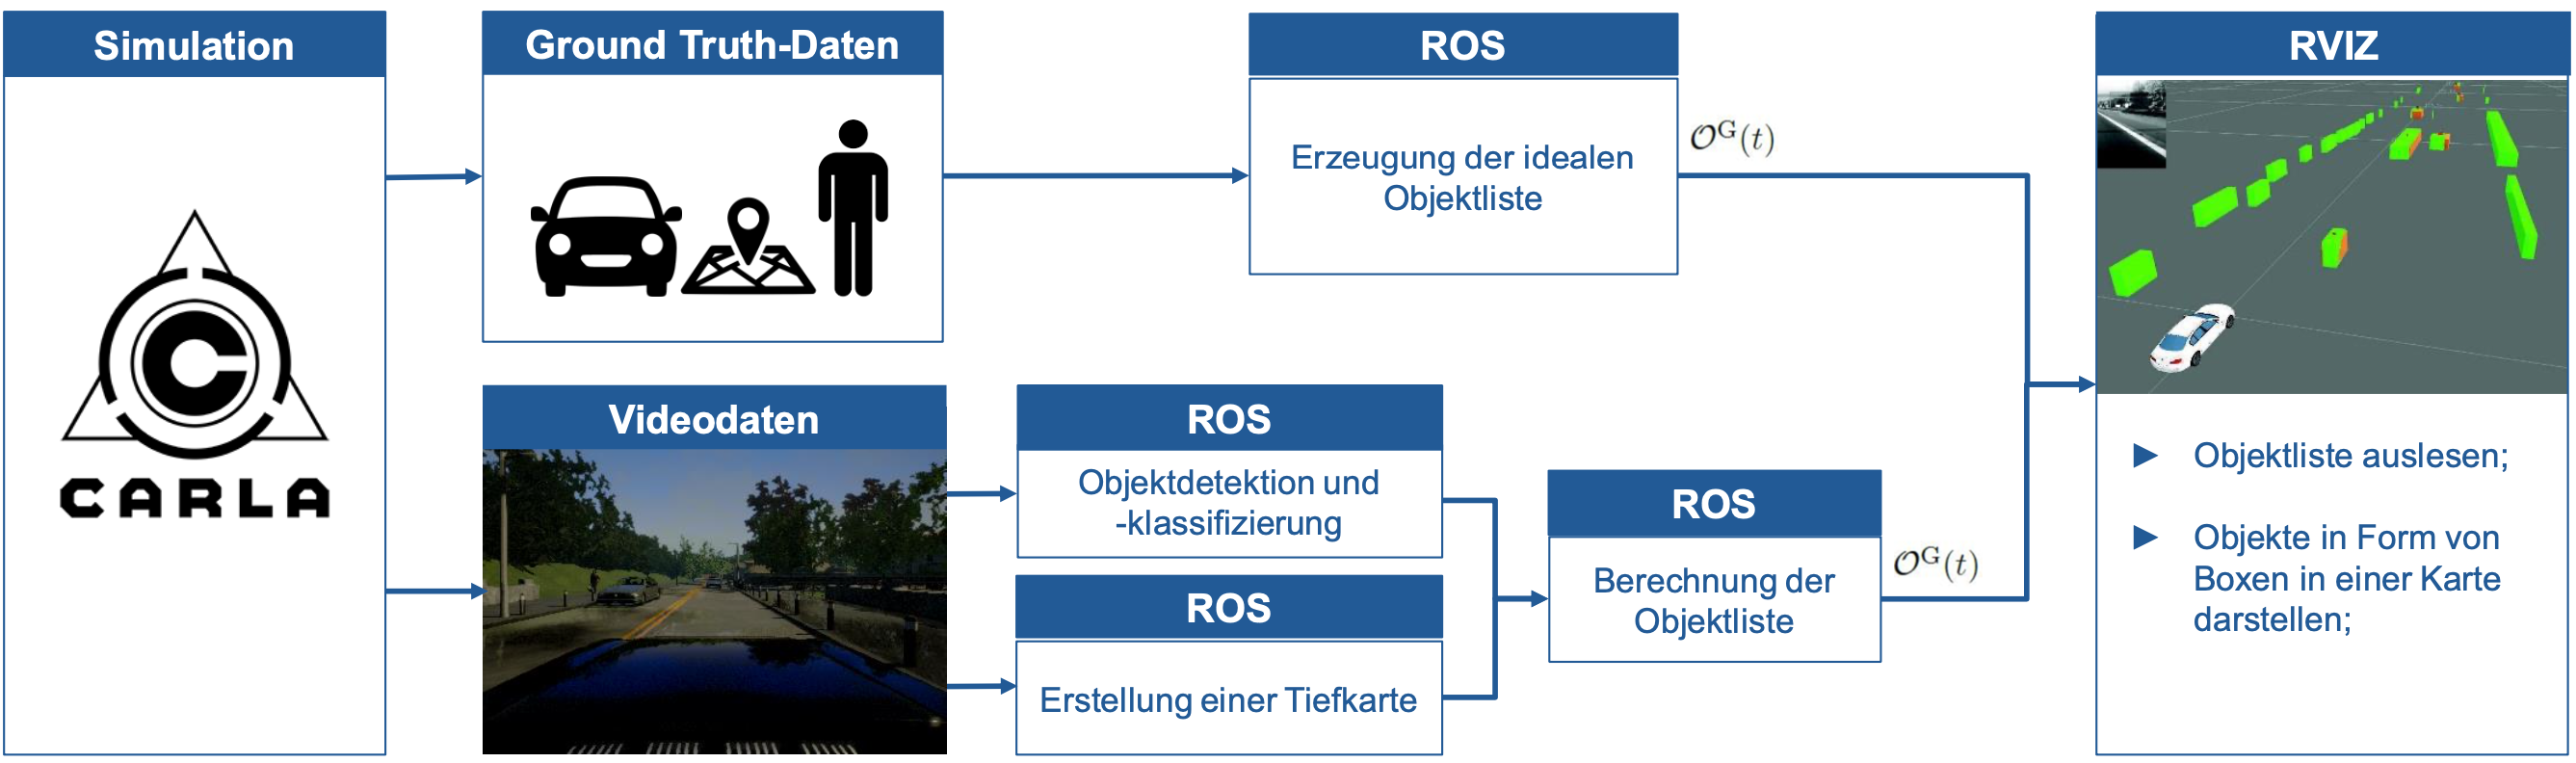
\includegraphics[width=2\linewidth]{images/Ueberblick}
%%	\captionof{figure}{My caption}
%%	\label{fig:mc-1}
%%\end{center}\newpage
%
%CARLA is an open-source urban driving simulator for autonomous driving research and supports flexible sensor suit and full control of all static and dynamic actors and maps \cite{Dosovitskiy17}. This offers the possibility to validate the camera data sets using different kind of camera-based algorithms for object detection or to train them quickly and easily. To evaluate the Ground-Truth Data of the simulation with the calculated algorithm objects, \ac{ROS} offers the possibility of sending the respective data streams using objects lists and evaluating them with a \ac{RVIZ} \cite{ROS}.
%In this work, an autonomous driving environment model visualization based on an object list level is presented by using a NCAP test scenario for testing automated driving systems. An analysis is made based on the \ac{YOLO} camera object detection algorithm compared to the Ground-Truth Data directly generated out of the environment simulation software model. !!!!HIER WUERDE ICH DIE OVERVIEW GRAFIK ERWAEHNEN UND DIREKT DARUNTER AM ENDE DER SEITE POSITIONIEREN, KANN ABER SCHWIERIG WERDEN, DA NOCH ABSTRACT FEHLT!!! \Cref{fig:Overview}
%
%
%
